\documentclass[final]{beamer}
\usepackage[ngerman]{babel}
\usepackage[utf8]{inputenc}
\usepackage[T1]{fontenc}
\usepackage{lmodern}
\usepackage{listings}
\usepackage{graphicx}
\usepackage{color}
\usepackage{amssymb}
\usepackage{transparent}

\definecolor{mygreen}{rgb}{0,0.6,0}
\definecolor{mygray}{rgb}{0.5,0.5,0.5}
\lstset{
  basicstyle=\footnotesize,			% the size of the fonts that are used for the code
  breakatwhitespace=false,			% sets if automatic breaks should only happen at whitespace
  breaklines=true,					% sets automatic line breaking
  captionpos=b,					% sets the caption-position to bottom
  commentstyle=\color{mygreen},		% comment style
  deletekeywords={...},				% if you want to delete keywords from the given language
  extendedchars=true,				% lets you use non-ASCII characters; for 8-bits encodings only, does not work with UTF-8
  frame=none,						% adds a frame around the code
  keepspaces=true,					% keeps spaces in text, useful for keeping indentation of code (possibly needs columns=flexible)
  keywordstyle=\color{blue},			% keyword style
  language=Java,					% the language of the code
  morekeywords={*,...},				% if you want to add more keywords to the set
  numbers=none,					% where to put the line-numbers; possible values are (none, left, right)
  rulecolor=\color{mygreen},			% if not set, the frame-color may be changed on line-breaks within not-black text (e.g. comments (green here))
  showspaces=false,					% show spaces everywhere adding particular underscores; it overrides 'showstringspaces'
  showstringspaces=false,			% underline spaces within strings only
  showtabs=false,					% show tabs within strings adding particular underscores
  stepnumber=1,					% the step between two line-numbers. If it's 1, each line will be numbered
  stringstyle=\color{red},				% string literal style
  tabsize=4,						% sets default tabsize to 2 spaces
  title=\lstname					% show the filename of files included with \lstinputlisting; also try caption instead of title
}

\newcommand{\ThemeFolder}{FSIBeamerTheme}
\RequirePackage{\ThemeFolder/beamerthemeFSI}
\lstset{language=Java}

\DeclareGraphicsExtensions{.pdf,.png}

\mode<presentation>

\title{Programmiervorkurs für Erstsemester}

\setbeamertemplate{title page}{
  \begin{center}
    \color{FSIblue}
      \resizebox{\textwidth}{!}{Programmiervorkurs}\\
      \vspace{0.3\baselineskip}
      \huge{Einführung in Java}\\
      \huge{Tag 4}
      \vfill
      \large{Tristan Wagner}\\
      \tiny{WS 2013/2014}
  \end{center}
}

\begin{document}

\lstset{tabsize=4}
\lstset{basicstyle=\small}
\lstset{language=java}

\begin{frame}
  \titlepage
\end{frame}

\begin{frame}
	\frametitle{Inhaltsübersicht Vorkurs}
	\begin{itemize}
	{\color{gray}
		\item {Tag 1: Variablen, Datentypen, Konvertierungen, Arithmetik, Netbeans, Einführung Debugging}
		\item {Tag 2: Boolesche Ausdrücke, Kommentare, If-Abfragen, Switch-Case, Weiterführung Debugging}
		\item {Tag 3: Arrays, (Do-)While-Schleife, For-Schleifen, Weiterführung Debugging}
		{\color{black}
		\item {Tag 4: (statische) Methoden, Attribute, Ausführung Debugging}
		}
	}
	\end{itemize}
\end{frame}

\section{Über mich}
\begin{frame}
	\frametitle{Über mich}
	\textbf{Tristan Wagner}
	\begin{itemize}
		\item{7. Semester Informatik}
		\item{aktiver Fachschafter}
		\item{Kassenwart des Fachschaftsvereins}
	\end{itemize}
\end{frame}

\section{Methoden}
\begin{frame}[containsverbatim]
	\frametitle{Beispiel ohne Methoden}
	\begin{lstlisting}
public class Main {
	public static void main() {
		for (int i = 1; i <= 10; i++) {
			System.out.println(i);
		}
		
		// weiterer Code
		
		for (int i = 1; i <= 10; i++) {
			System.out.println(i);
		}
	}
}
	\end{lstlisting}
\end{frame}

\subsection{Warum?}
\begin{frame}
	\frametitle{Warum?}
	\textbf{Probleme?}
	\begin{itemize}
		\item{zeitaufwändig}
		\item{(zu) viel Code}
		\item{unübersichtlich}
		\item{Änderungen kosten noch mehr Zeit}
		\item{Code oft nicht wiederverwendbar}
		\item{Arbeitsteilung kaum möglich}
	\end{itemize}
	\pause
	\vspace{\baselineskip}
	\textbf{Lösungen?}
	\pause
	\begin{itemize}
		\item{ähnlichen Code auslagern}
		\item{wiederverwendbaren Code schreiben}
		\item{\textbf{Methoden!}}
	\end{itemize}
\end{frame}

\begin{frame}[containsverbatim]
	\frametitle{Beispiel mit Methoden}
	\begin{lstlisting}
public class Main {
	public static void main () {
		zaehlBisZehn();
		
		// weiterer Code
		
		zaehlBisZehn();
	}
	
	public static void zaehlBisZehn() {
		for (int i = 1; i <= 10; i++) {
			System.out.println(i);
		}
	}
}
	\end{lstlisting}
\end{frame}

\subsection{Wie?}
\begin{frame}[containsverbatim]
	\frametitle{Kopf der Methode}
	\begin{lstlisting}
public static void zaehlBisZehn () { 
	...
}
	\end{lstlisting}
	\begin{itemize}
		\item{\textbf{public static} immer am Anfang (wird im Vorkurs nicht behandelt)}
		\item{\textbf{Methodenname} vor den runden Klammern}
	\end{itemize}
\end{frame}

\begin{frame}[containsverbatim]
	\frametitle{Aufruf einer Methode}
	\begin{lstlisting}
public static void Main () {
	zaehlBisZehn();
}
	\end{lstlisting}
	\begin{itemize}
		\item{Methodenname}
		\item{()}
		\item{;}
	\end{itemize}
\end{frame}

\subsection{Mehr!}
\begin{frame}
	\frametitle{Methoden können mehr!}
	\begin{itemize}
		\item{Beim Methodenaufruf können zusätzliche Informationen (= Parameter) an die Methode übergeben werden}
		\item{Methoden können Informationen an den Aufrufer zurück geben}
		\item{Methoden können sich selbst aufrufen (= Rekursion) (nicht Teil des Vorkurses)}
	\end{itemize}
\end{frame}

\subsubsection{Methoden mit Parameter}
\begin{frame}[containsverbatim]
	\frametitle{Beispiel ohne Methoden}
	\begin{lstlisting}[escapechar=!]
public class Main () {
	public static void main() {
		for (int i = 1; i <= !\color{red}\textbf{9}!; i++) {
			System.out.println(i);
		}
		
		// weiterer Code
		
		for (int i = 1; i <= !\color{red}\textbf{10}!; i++) {
			System.out.println(i);
		}
	}
}
	\end{lstlisting}
\end{frame}

\begin{frame}[containsverbatim]
	\frametitle{Beispiel mit Methoden}
	\begin{lstlisting}[escapechar=!]
public class Main() {
	public static void main() {
		zaehleBis(!\color{red}\textbf{9}!);
		
		// weiterer Code
		
		zaehleBis(!\color{red}\textbf{10}!);
	}

	public static void zaehleBis(!\textbf{\color{blue}int \color{red}z}!) {
		for (int i = 1; i <= !\color{red}\textbf{z}!; i++) {
			System.out.println(i);
		}
	}
}
	\end{lstlisting}
\end{frame}

\begin{frame}[containsverbatim]
	\frametitle{Kopf der Methode}
	\begin{lstlisting}[escapechar=!]
public static void zaehleBis(!\color{blue}int \color{red}z!) {
	...
}
	\end{lstlisting}
	\begin{itemize}
		\item{In die runden Klammern kommen die Paramter}
		\item{Parameter werden mit Komma getrennt:
			\begin{lstlisting}[escapechar=!]
(!\color{blue}int \color{red}a!, !\color{blue}boolean \color{red}b!, !\color{blue}double \color{red}c!)
			\end{lstlisting}
		}
		\item{Ein Parameter besteht aus {\color{blue}Datentyp} und \color{red}Bezeichner}
	\end{itemize}
\end{frame}

\begin{frame}[containsverbatim]
	\frametitle{Aufruf}
	\begin{lstlisting}[escapechar=!]
pulic static void main() {
	zaehleBis(!\color{red}9!);
	zaehleBis(!\color{red}10!);
}
	\end{lstlisting}
	\begin{itemize}
		\item{Parameter, die man übergeben möchte, durch Komma getrennt in die Runden Klammern}
	\end{itemize}
\end{frame}

\begin{frame}[containsverbatim]
	\frametitle{Was passiert?}
	\begin{itemize}
		\item{
			\begin{lstlisting}[escapechar=!]
zaehleBis(!\color{red}9!);
			!\vspace{\baselineskip}!
public static void zaehleBis(!\color{blue}int \color{red}z!) {
	// z wird der Wert 9 zugewiesen
}
			\end{lstlisting}
		}
		\vspace{\baselineskip}
		\item{
			\begin{lstlisting}[escapechar=!]
zaehleBis(!\color{red}10!);
			!\vspace{\baselineskip}!
public static void zaehleBis(!\color{blue}int \color{red}z!) {
	// z wird der Wert 10 zugewiesen
}
			\end{lstlisting}
		}
	\end{itemize}
\end{frame}

\begin{frame}[containsverbatim]
	\frametitle{Beispiel mit 2 Parametern}
	\begin{lstlisting}[escapechar=!]
public class Main {
	public static void main() {
		zaehleVonBis(!\color{blue}1!, !\color{red}9!);
		// weiterer Code
		zaehleVonBis(!\color{blue}5!, !\color{red}10!);
	}
	
	public static void 
		zaehleVonBis(int !\color{blue}v!, int !\color{red}b!) {
		for (int i = !\color{blue}v!; i <= !\color{red}b!; i++) {
			System.out.println(i);
		}
	}
}
	\end{lstlisting}
\end{frame}

\subsubsection{Methoden mit Rückgabewert}
\begin{frame}[containsverbatim]
	\frametitle{Beispiel mit Rückgabewert}
	\begin{lstlisting}[escapechar=!]
public class Main {
	public static void main() {
		!\color{blue}int! !\color{red}x! = zaehleVonBis(1, 9);
	}
	
	public static !\color{blue}int! 
		zaehleVonBis(int v, int b) {
		for (int i = v; i <= b; i++) {
			System.out.println(i);
		}
		
		!\color{blue}return! !\color{red}b - v + 1!;
	}
}
	\end{lstlisting}
\end{frame}

\begin{frame}[containsverbatim]
	\frametitle{Kopf der Methode}
	\begin{lstlisting}[escapechar=!]
public static !\color{blue}int! zaehleVonBis(int v, int b) {
	...
	!\color{blue}return! !\color{red}b - v + 1!;
}
	\end{lstlisting}
	\begin{itemize}
		\item{Möchte man keinen Wert zurück geben, so kommt nach \textbf{static} das Schlüsselwort \color{blue}void}
		\item{Ansonsten wird {\color{blue}void} durch den gewünschten Datentyp ersetzt}
		\item{Mit {\color{blue}return} wird der Wert zurückgegeben. Das {\color{blue}return} ist Pflicht und muss erreicht werden}
	\end{itemize}
\end{frame}

\begin{frame}[containsverbatim]
	\frametitle{Was passiert?}
	\begin{lstlisting}[escapechar=!]
!\color{blue}int! !\color{red}x! = zaehleVonBis(1, 9);
	\end{lstlisting}
	\begin{itemize}
		\item{Rechte Seite von "\textbf{=}"\ wird zuerst ausgewertet
			\begin{itemize}
				\item{zaehleVonBis(1, 9);}
			\end{itemize}
		}
	\end{itemize}
	\begin{lstlisting}[escapechar=!]
public static !\color{blue}int! zaehleVonBis(int v, int b) {
	...
	!\color{blue}return! !\color{red}b - v + 1!;
}
	\end{lstlisting}
	\begin{itemize}
		\item{v = 1, b = 9
			\begin{itemize}
				\item{return 9 - 1 + 1 = 9}
					\begin{itemize}
						\item{9 wird zurückgegeben}
					\end{itemize}
			\end{itemize}
		}
		\item{{\color{red}x} wird der Wert 9 zugewiesen}
	\end{itemize}
\end{frame}

\begin{frame}[containsverbatim]
	\frametitle{Generell}
	\begin{lstlisting}[escapechar=!]
public static !\color{blue}Rückgabetyp! !\color{green}Name! (!\color{red}Parameter!) {
	// Methodenrumpf
	!\color{blue}return! ... ; 
}
	\end{lstlisting}
	\begin{itemize}
		\item{Wenn der {\color{blue}Rückgabetyp} \textbf{void} ist, darf das {\color{blue}return} keinen Rückgabewert haben und ist optional}
	\end{itemize}
\end{frame}

\section{Klassenvariablen}
\begin{frame}[containsverbatim]
	\frametitle{Beispiel ohne Klassenvariablen}
	\begin{lstlisting}[escapechar=!]
public class Main {
	public static void main() {
		!\color{blue}int! !\color{red}x! = zaehleVonBis(1, 9);
	}
	
	public static !\color{blue}int! 
		zaehleVonBis(int v, int b) {
		for (int i = v; i <= b; i++) {
			System.out.println(i);
		}
		
		boolean wurdeAusgegeben = b >= v;
		
		!\color{blue}return! !\color{red}b - v + 1!;
	}
}
	\end{lstlisting}
\end{frame}

\subsection{Warum?}
\begin{frame}
	\frametitle{Warum?}
	\textbf{Probleme}
	\begin{itemize}
		\item{Methoden können nur einen Wert zurückgeben}
		\item{Eine Methode kann nicht auf Daten aus anderen Methoden zugreifen}
	\end{itemize}
	\vspace{\baselineskip}
	\pause
	\textbf{Lösungen}
	\pause
	\begin{itemize}
		\item{\textbf{Klassenvariablen}
			\begin{itemize}
				\item{mit Bedacht verwenden!}
			\end{itemize}
		}
	\end{itemize}
\end{frame}
	
\subsection{Wie?}
\begin{frame}[containsverbatim]
	\frametitle{Beispiel mit Klassenvariablen}
	\begin{lstlisting}[escapechar=!]
public class Main {
	!\color{blue}public static boolean! !\color{red}wurdeAusgegeben!;
	public static void main() {
		int x = zaehleVonBis(1, 9);
		System.out.println(wurdeAusgegeben);
	}
	
	public static int 
		zaehleVonBis(int v, int b) {
		for (int i = v; i <= b; i++) {
			System.out.println(i);
		}
		!\color{red}wurdeAusgegeben! = b >= v;
		return b - v + 1;
	}
}
	\end{lstlisting}
\end{frame}

\begin{frame}[containsverbatim]
	\frametitle{Deklaration von Klassenvariablen}
	\begin{itemize}
		\item{Deklaration direkt nach Klassendeklaration}
		\item{\textbf{public static} {\color{blue}Datentyp} {\color{red}Bezeichner};}
		\item{sichtbar in der ganzen Klasse}
		\item{Ohne manuelle Zuweisung wird der Defaultwert zugewiesen}
		\item{Beispiel:
			\begin{lstlisting}[escapechar=!]
public static !\color{blue}boolean! !\color{red}wurdeAusgegeben!;
			\end{lstlisting}
		}
	\end{itemize}
\end{frame}

\section{Java-Doc}
\begin{frame}
	\frametitle{JavaDoc}
	JavaDoc bietet einfache Kommentar für Klassen und Methoden (Ausgabe erfolgt in html)
	\begin{itemize}
		\item{Genereller Aufbau}
			\begin{itemize}
				\item{Mehrzeiliges Kommentar (Mit zwei sternen) /**...*/}
			\end{itemize}
		\item{@Author}
			\begin{itemize}
				\item{Gibt den Author einer Datei oder Klasse an}
			\end{itemize}
		\item{@Param}
			\begin{itemize}
				\item{Parameter die einer Methode übergeben werden}
			\end{itemize}
		\item{@Return}
			\begin{itemize}
				\item{Definiert den Rückgabewert der Funktion}
			\end{itemize}
	\end{itemize}
\end{frame}

\section{Exceptions}
\begin{frame}
	\frametitle{Exceptions}
	\textbf{Häufige Exceptions}
	\begin{itemize}
		\item{NullPointerException}
			\begin{itemize}
				\item{Zugriff auf einen Variable in der \color{blue}null \color{black} steht}
			\end{itemize}
		\item{ArrayIndexOutOfBoundsException}
			\begin{itemize}
				\item{Zugriff auf ein Arrayelement außerhalb der Arraygrenzen}
			\end{itemize}
		\item{ArithmeticException}
			\begin{itemize}
				\item{Division durch 0}
			\end{itemize}
	\end{itemize}
\end{frame}

\section{Aufgabe}
\begin{frame}
	\frametitle{Vorstellung der Aufgabe}
	\begin{columns}[T]
		\column{0.5\textwidth}
			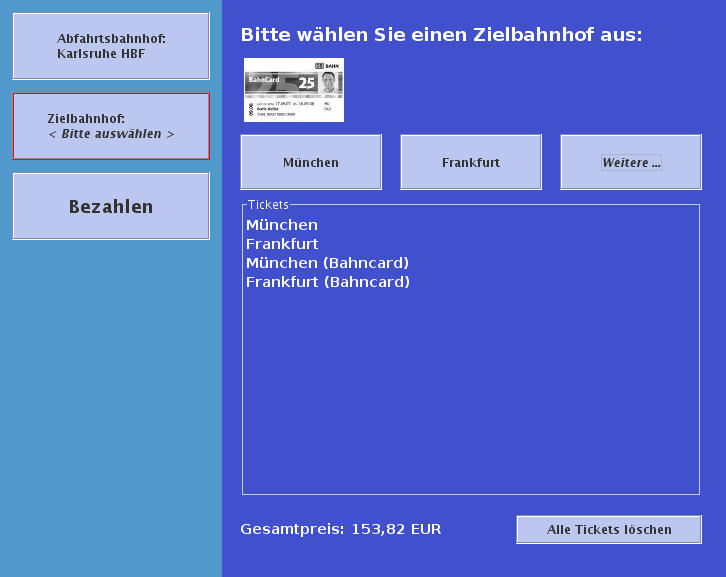
\includegraphics[width=\textwidth]{gfx/bahnticketautomat_buchen}
		\column{0.5\textwidth}
			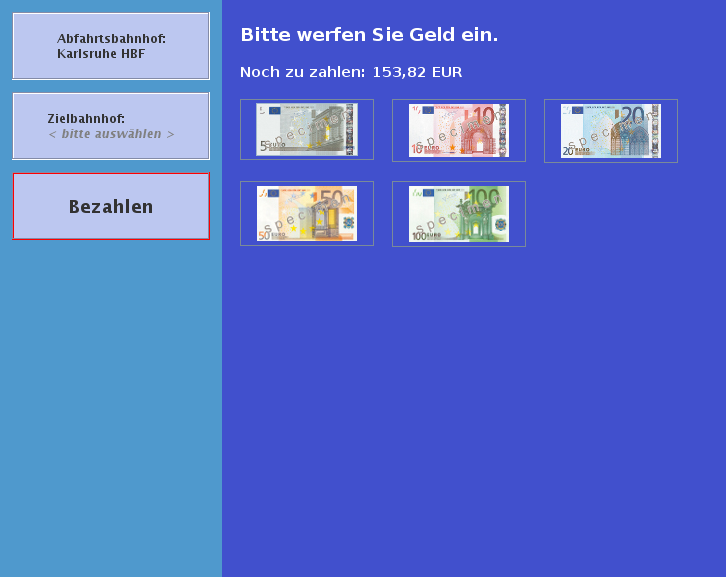
\includegraphics[width=\textwidth]{gfx/bahnticketautomat_bezahlen}
	\end{columns}
	\vspace{\baselineskip}
	\begin{columns}[T]
		\column{0.5\textwidth}
			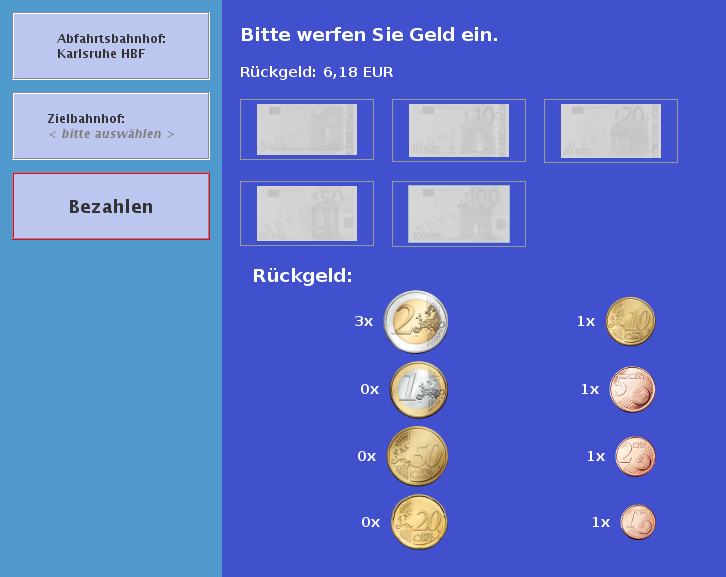
\includegraphics[width=\textwidth]{gfx/bahnticketautomat_rueckgeld}
		\column{0.5\textwidth}
		\pause
			
\includegraphics[width=\textwidth]{gfx/Wait-what-meme-rage-face.jpg}
	\end{columns}
\end{frame}

\subsection{Methoden}
\begin{frame}
	\frametitle{Methoden}
	\begin{itemize}
		\item{{\color{blue}public static} String[] \textbf{addNewTicket}(String[] oldTickets, String newTicket, {\color{blue}boolean} bahncard)}
		\item{{\color{blue}public static void} \textbf{calculateNewSum}({\color{blue}int} distance, {\color{blue}boolean} bahncard)}
		\item{{\color{blue}public static double} \textbf{getSum}()}
		\item{{\color{blue}public static void} \textbf{resetSum}()}
		\item{{\color{blue}public static void} \textbf{beginPayment}()}
		\item{{\color{blue}public static void} \textbf{insertMoney}({\color{blue}int} amount)}
		\item{{\color{blue}public static double} \textbf{getAmountLeft}()}
		\item{{\color{blue}public static boolean} \textbf{isAmountLeft}()}
		\item{{\color{blue}public static double} \textbf{getChangeAmount}()}
		\item{{\color{blue}public static int}[] \textbf{getChangeCoins}()}
	\end{itemize}
\end{frame}

\subsubsection{addNewTicket}
\begin{frame}
	\frametitle{addNewTicket}
	\begin{itemize}
		\item{Parameter:}
			\begin{itemize}
				\item{oldTickets: String Array enthält die alten Tickets}
				\item{newTickets: String}
			\end{itemize}
	\end{itemize}
\end{frame}

\subsubsection{calculateNewSum}
\begin{frame}
	\frametitle{calculateNewSum}
	\begin{itemize}
		\item{}
	\end{itemize}
\end{frame}

\subsubsection{getSum}
\begin{frame}
	\frametitle{getSum}
	\begin{itemize}
		\item{}
	\end{itemize}
\end{frame}

\subsubsection{resetSum}
\begin{frame}
	\frametitle{resetSum}
	\begin{itemize}
		\item{}
	\end{itemize}
\end{frame}

\subsubsection{beginPayment}
\begin{frame}
	\frametitle{beginPayment}
	\begin{itemize}
		\item{}
	\end{itemize}
\end{frame}

\subsubsection{insertMoney}
\begin{frame}
	\frametitle{insertMoney}
	\begin{itemize}
		\item{}
	\end{itemize}
\end{frame}

\subsubsection{getAmountLeft}
\begin{frame}
	\frametitle{getAmountLeft}
	\begin{itemize}
		\item{}
	\end{itemize}
\end{frame}

\subsubsection{getChangeAmount}
\begin{frame}
	\frametitle{getChangeAmount}
	\begin{itemize}
		\item{}
	\end{itemize}
\end{frame}

\subsubsection{addNewTicket}
\begin{frame}
	\frametitle{addNewTicket}
	\begin{itemize}
		\item{}
	\end{itemize}
\end{frame}

\subsubsection{getChangeCoins}
\begin{frame}
	\frametitle{getChangeCoins}
	\begin{itemize}
		\item{}
	\end{itemize}
\end{frame}

\section{Quellen \& Lizenz}
\begin{frame}
	\frametitle{Quellen und Lizenz}
	\begin{center}
		
\includegraphics[width=250px]{gfx/fsi}
	\end{center}
	\begin{itemize}
		\item{Original von Samuel Zeitvogel}
		\item{Überarbeitet 2012 von Daniel Hoff}
		\item{Überarbeitet 2013 von Tristan Wagner}
	\end{itemize}
\end{frame}

\end{document}
